\documentclass{article}\usepackage[]{graphicx}\usepackage[]{color}
% maxwidth is the original width if it is less than linewidth
% otherwise use linewidth (to make sure the graphics do not exceed the margin)
\makeatletter
\def\maxwidth{ %
  \ifdim\Gin@nat@width>\linewidth
    \linewidth
  \else
    \Gin@nat@width
  \fi
}
\makeatother

\definecolor{fgcolor}{rgb}{0.345, 0.345, 0.345}
\newcommand{\hlnum}[1]{\textcolor[rgb]{0.686,0.059,0.569}{#1}}%
\newcommand{\hlstr}[1]{\textcolor[rgb]{0.192,0.494,0.8}{#1}}%
\newcommand{\hlcom}[1]{\textcolor[rgb]{0.678,0.584,0.686}{\textit{#1}}}%
\newcommand{\hlopt}[1]{\textcolor[rgb]{0,0,0}{#1}}%
\newcommand{\hlstd}[1]{\textcolor[rgb]{0.345,0.345,0.345}{#1}}%
\newcommand{\hlkwa}[1]{\textcolor[rgb]{0.161,0.373,0.58}{\textbf{#1}}}%
\newcommand{\hlkwb}[1]{\textcolor[rgb]{0.69,0.353,0.396}{#1}}%
\newcommand{\hlkwc}[1]{\textcolor[rgb]{0.333,0.667,0.333}{#1}}%
\newcommand{\hlkwd}[1]{\textcolor[rgb]{0.737,0.353,0.396}{\textbf{#1}}}%
\let\hlipl\hlkwb

\usepackage{framed}
\makeatletter
\newenvironment{kframe}{%
 \def\at@end@of@kframe{}%
 \ifinner\ifhmode%
  \def\at@end@of@kframe{\end{minipage}}%
  \begin{minipage}{\columnwidth}%
 \fi\fi%
 \def\FrameCommand##1{\hskip\@totalleftmargin \hskip-\fboxsep
 \colorbox{shadecolor}{##1}\hskip-\fboxsep
     % There is no \\@totalrightmargin, so:
     \hskip-\linewidth \hskip-\@totalleftmargin \hskip\columnwidth}%
 \MakeFramed {\advance\hsize-\width
   \@totalleftmargin\z@ \linewidth\hsize
   \@setminipage}}%
 {\par\unskip\endMakeFramed%
 \at@end@of@kframe}
\makeatother

\definecolor{shadecolor}{rgb}{.97, .97, .97}
\definecolor{messagecolor}{rgb}{0, 0, 0}
\definecolor{warningcolor}{rgb}{1, 0, 1}
\definecolor{errorcolor}{rgb}{1, 0, 0}
\newenvironment{knitrout}{}{} % an empty environment to be redefined in TeX

\usepackage{alltt}

\usepackage{float}
\usepackage{mathtools}
\usepackage{geometry}
\geometry{legalpaper, margin=2in}


\title{My Second \texttt{knitr} Document}
\author{Jane Doe}
\date{\today}
\IfFileExists{upquote.sty}{\usepackage{upquote}}{}
\begin{document}


\maketitle

\section{Introduction}
We want to know if iris sepal length is correlated with iris petal width or petal length.

\section{Methods}
To examine the relationship between iris sepal length and petal width and petal length, we used the following linear regression model:

\begin{align}
y_i&=\beta_0+\beta_1x_{i,1}+\beta_2x_{i,2}+\epsilon_i, \notag \\
\epsilon_i &\sim \text{Normal}(0,\sigma^2), \notag
\end{align}

where $y_i$ represents iris sepal length for the $i=1,\ldots,n$ flowers, $x_{i,1}$ represents the $i^{th}$ flower's average petal width, and $x_{i,2}$ represents the $i^{th}$ flower's average petal length. To estimate model parameters, we used \texttt{R} statistical software. The \texttt{R} script is shown, below.
\subsection{\texttt{R} script for iris data}

\begin{knitrout}
\definecolor{shadecolor}{rgb}{0.969, 0.969, 0.969}\color{fgcolor}\begin{kframe}
\begin{alltt}
\hlcom{###}
\hlcom{### Load the datasets library which contains the iris data}
\hlcom{###}

\hlkwd{library}\hlstd{(datasets)}
\hlkwd{data}\hlstd{(iris)}

\hlcom{###}
\hlcom{### set the response variable to the object called "y"}
\hlcom{###}

\hlstd{y}\hlkwb{=}\hlstd{iris}\hlopt{$}\hlstd{Sepal.Length}

\hlcom{###}
\hlcom{### Define the predictor variables}
\hlcom{###}

\hlstd{x1}\hlkwb{=}\hlstd{iris}\hlopt{$}\hlstd{Petal.Length}
\hlstd{x2}\hlkwb{=}\hlstd{iris}\hlopt{$}\hlstd{Petal.Width}

\hlcom{###}
\hlcom{### Fit the linear model to the data}
\hlcom{###}

\hlstd{linMod}\hlkwb{=}\hlkwd{lm}\hlstd{(y}\hlopt{~}\hlstd{x1}\hlopt{+}\hlstd{x2)}
\hlstd{betas}\hlkwb{=}\hlkwd{coef}\hlstd{(linMod)}
\hlstd{std.er}\hlkwb{=}\hlkwd{coef}\hlstd{(}\hlkwd{summary}\hlstd{(linMod))[,} \hlnum{2}\hlstd{]}
\hlstd{sigma}\hlkwb{=}\hlkwd{sqrt}\hlstd{(}\hlkwd{deviance}\hlstd{(linMod)}\hlopt{/}\hlkwd{df.residual}\hlstd{(linMod))}
\end{alltt}
\end{kframe}
\end{knitrout}

\section{Results}
\subsection{Parameter Estimates}
The estimated intercept of our model, $\beta_0$, was 4.19. Thus, the expected sepal length for an iris with mean petal length equal to zero, and mean petal width equal to zero was 4.19. The estimated regression parameter for petal length, $\beta_1$,  was 0.54. Thus, as petal length increased by one unit, the expected value of sepal length incresed by 0.54. 

Our fitted model is:
\begin{align}
y_i&=4.19+0.54x_{i,1}+-0.32x_{i,2}+\epsilon_i, \notag \\
\epsilon_i &\sim \text{Normal}(0,0.4^2), \notag
\end{align}

\subsection{Figures}
To see the marginal relationship between $y_i$ and $x_{i,1}$ and $x_{i,2}$, see Fig. \ref{fig:marginals}

\begin{figure}
\begin{knitrout}
\definecolor{shadecolor}{rgb}{0.969, 0.969, 0.969}\color{fgcolor}\begin{kframe}
\begin{alltt}
\hlcom{###}
\hlcom{### Plot the relationship between the response variable}
\hlcom{### and each predictor variable}
\hlcom{###}

\hlkwd{par}\hlstd{(}\hlkwc{mfrow}\hlstd{=}\hlkwd{c}\hlstd{(}\hlnum{2}\hlstd{,}\hlnum{1}\hlstd{),}\hlkwc{mar}\hlstd{=}\hlkwd{c}\hlstd{(}\hlnum{4}\hlstd{,}\hlnum{4}\hlstd{,}\hlnum{2}\hlstd{,}\hlnum{2}\hlstd{))}

\hlcom{## Top figure}
\hlkwd{plot}\hlstd{(x1,y)}
\hlstd{x1.pred}\hlkwb{=}\hlkwd{seq}\hlstd{(}\hlkwd{range}\hlstd{(x1)[}\hlnum{1}\hlstd{],}\hlkwd{range}\hlstd{(x1)[}\hlnum{2}\hlstd{],}\hlkwc{length.out}\hlstd{=}\hlnum{10}\hlstd{)}
\hlstd{x2.mean}\hlkwb{=}\hlkwd{mean}\hlstd{(x2)}

\hlstd{y.pred1}\hlkwb{=}\hlstd{betas[}\hlnum{1}\hlstd{]}\hlopt{+}\hlstd{betas[}\hlnum{2}\hlstd{]}\hlopt{*}\hlstd{x1.pred}\hlopt{+}\hlstd{betas[}\hlnum{3}\hlstd{]}\hlopt{*}\hlstd{x2.mean}
\hlkwd{lines}\hlstd{(x1.pred,y.pred1,}\hlkwc{col}\hlstd{=}\hlnum{2}\hlstd{,}\hlkwc{lwd}\hlstd{=}\hlnum{3}\hlstd{)}

\hlcom{## Bottom figure}
\hlkwd{plot}\hlstd{(x2,y)}
\hlstd{x1.mean}\hlkwb{=}\hlkwd{mean}\hlstd{(x1)}
\hlstd{x2.pred}\hlkwb{=}\hlkwd{seq}\hlstd{(}\hlkwd{range}\hlstd{(x2)[}\hlnum{1}\hlstd{],}\hlkwd{range}\hlstd{(x2)[}\hlnum{2}\hlstd{],}\hlkwc{length.out}\hlstd{=}\hlnum{10}\hlstd{)}

\hlstd{y.pred2}\hlkwb{=}\hlstd{betas[}\hlnum{1}\hlstd{]}\hlopt{+}\hlstd{betas[}\hlnum{2}\hlstd{]}\hlopt{*}\hlstd{x1.mean}\hlopt{+}\hlstd{betas[}\hlnum{3}\hlstd{]}\hlopt{*}\hlstd{x2.pred}
\hlkwd{lines}\hlstd{(x2.pred,y.pred2,}\hlkwc{col}\hlstd{=}\hlnum{2}\hlstd{,}\hlkwc{lwd}\hlstd{=}\hlnum{3}\hlstd{)}
\end{alltt}
\end{kframe}
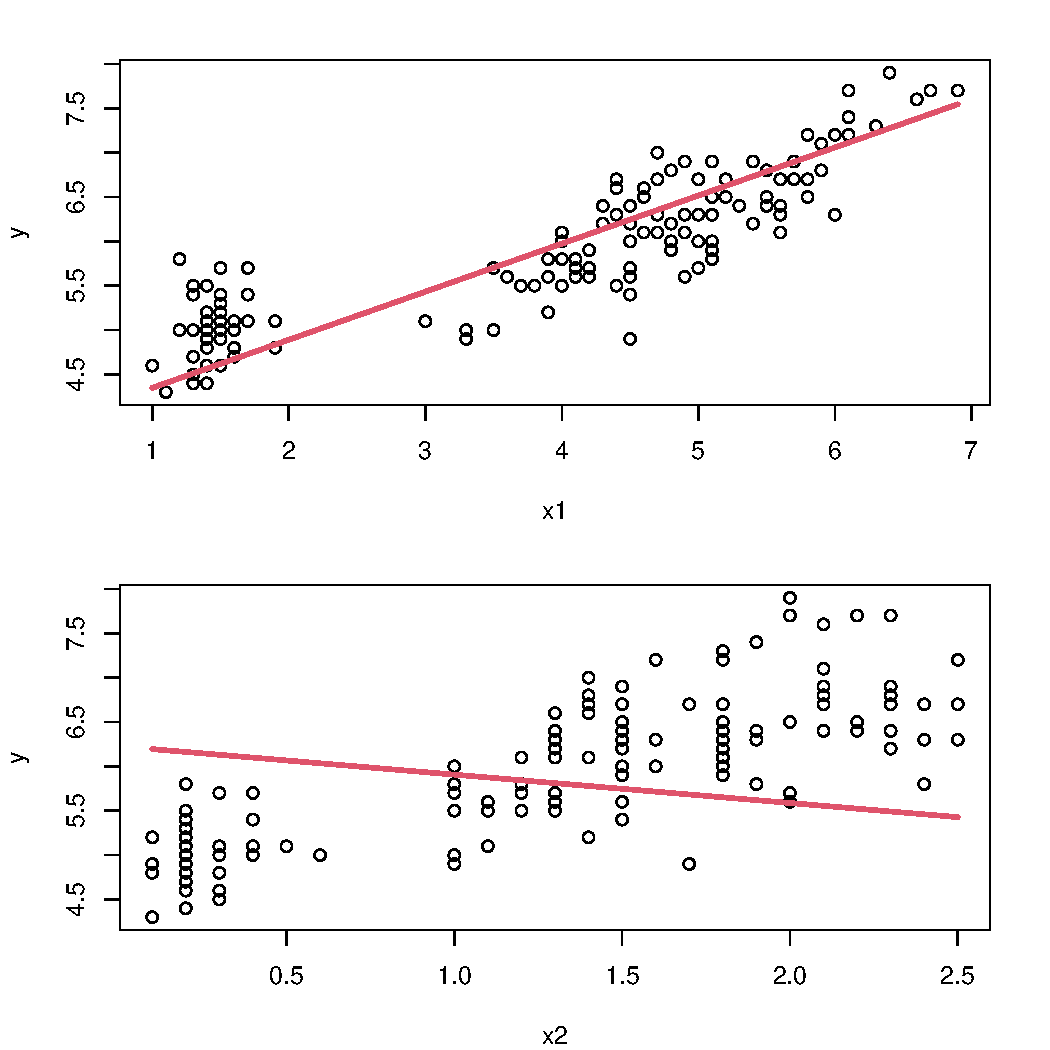
\includegraphics[width=\maxwidth]{figure/chunk2-1} 

\end{knitrout}

\caption{Marginal plot of the relationship between response variable and predictors.}
\label{fig:marginals}
\end{figure}

\subsection{Tables}
To see the parameter estimates and associated standard errors see Table \ref{tab:estimates}.

\begin{table}[H]
%\centering
\caption{Parameter estimates and SE of parameters from our fitted model.}
\begin{tabular}[t]{ l l l }
\hline
Parameter & Estimate & SE \\
\hline
 $\beta_0$ & 4.19 & 0.1 \\ 
 $\beta_1$ & 0.54 & 0.07 \\  
 $\beta_2$ & -0.32 & 0.16 \\
 $\sigma^2$ & 0.4$^2$ & - \\
 \hline
 \end{tabular}
\label{tab:estimates}
\end{table}

\section{Discussion}
Discuss the results here...

\end{document}
